\documentclass[10pt,twocolumn]{article}
	
\usepackage{myfontstyle}
\usepackage{mypackages}
\usepackage{mymacros}
\usepackage{mycommands}
\usepackage{textgreek}

\begin{document}
\thispagestyle{fancy1}

%%% Title and Abstract------------------------
\twocolumn[
\begin{center}
	\hrule
	\vspace{3pt}
	% Title:
	{\sffamily\bfseries\Large
		Report for Laboratory Three: RC Circuit Response
	} \\
	{\color{gray}
		\vspace{3pt}
		\hrule
		\vspace{3pt}
	}
	{
		\hspace*{\fill}
		Austin Piper
		\hspace*{\fill}
		Alex Blakley
		\hspace*{\fill}
		Irfan Ahmed
		\hspace*{\fill}
%		Fourth Author    % uncomment these two lines if there's a fourth author
%		\hspace*{\fill}
	}\\
	\vspace{3pt}
	{\itshape
		\hspace*{\fill}
		Department of Mechanical Engineering, Saint Martin's University
		\hspace*{\fill} \\
		\hspace*{\fill}
		ME/EE 316---Mechatronics \& Measurements Laboratory
		\hspace*{\fill}
	}\\
	\vspace{3pt}
	{
		\hspace*{\fill}
		\today{} % today's date ... can type manually instead
		\hspace*{\fill}
	}
	\vspace{3pt}
	{\color{gray}\hrule}
%	\vspace{2pt}
\end{center}
% Abstract:
\begin{adjustwidth}{1.5in}{1.5in}
{\small
\noindent\textbf{Abstract.} \hspace{1em}
	The purpose of this lab was to view and measure the response of the voltage across a capacitor in a RC circuit. After building the circuit on a breadboard we sent 1 volt across the completed circuit and we used the myRIO microcontroller in order to record the results. The output voltage and resulting graphs can be used to find the time constant.
}
\end{adjustwidth}
\vspace{9pt}
\hrule
\vspace{1\baselineskip}
]

%%% Body -------------------------

\section{Introduction} 
\label{sec:introduction}

There are many variations of circuits used in the world of electronics in order to accomplish and power useful machines. The common RC circuit is used in devices like pacemakers, noise cancelling products, and timing circuits. These types of circuits are used because they can filter signals, blocking some and allowing others to pass through and therefore they are effective in their usage. 

In this lab, we built a basic RC circuit on a breadboard with a single 100 kΩ resistor and a 10 µF capacitor. We hooked up the myRIO to the breadboard and, with the full circuit completed and grounded using jumper wires, we applied a DC voltage across the capacitor and the measurements were taken of both the source voltage and output voltage.  The advantage of using the myRIO is that we could pair this technology with the LabVIEW program in order to have a graph drafted, in real time, of both of the data streams we require in order to deepen our understanding of how the RC circuit reacts to a constant voltage over time. 



\section{Materials and Methods}

This experiment started with the building of a circuit that had a 100 kΩ resistor and a 10 µF capacitor in series using a breadboard and jumper wires. Using a multimeter, both the capacitor and resistor were measured in order to ensure they, indeed, had the desired value of capacitance and resistance we needed for the experiment. After the myRIO was connected to our circuit we then began setting up the LabVIEW program in order to both control the source voltage supplied across the capacitor and to measure the output voltage over time. Using LabVIEW, we were able to grab the data and create a graph that showed both of the aforementioned voltages after about 6 time constants (6RC).
\section{Results}
\label{sec:results}

   
By conducting a circuit analysis of our circuit seen in \autoref{fig:circuit},
we found the equation for voltage across the capacitor. Using the that equation we were able to derive the equation for τ. Once we had our equations we used the data collected from LABVIEW and plotted our Vc in \autoref{fig:VC}.
On the same plot we compared the Vs and Vo vs time \autoref{fig:RCgraph} then after linearizing our data we were able to find out time constant value τ = 1.01325. \autoref{fig:Linear}




 


\begin{figure}[bt]
	\centering
	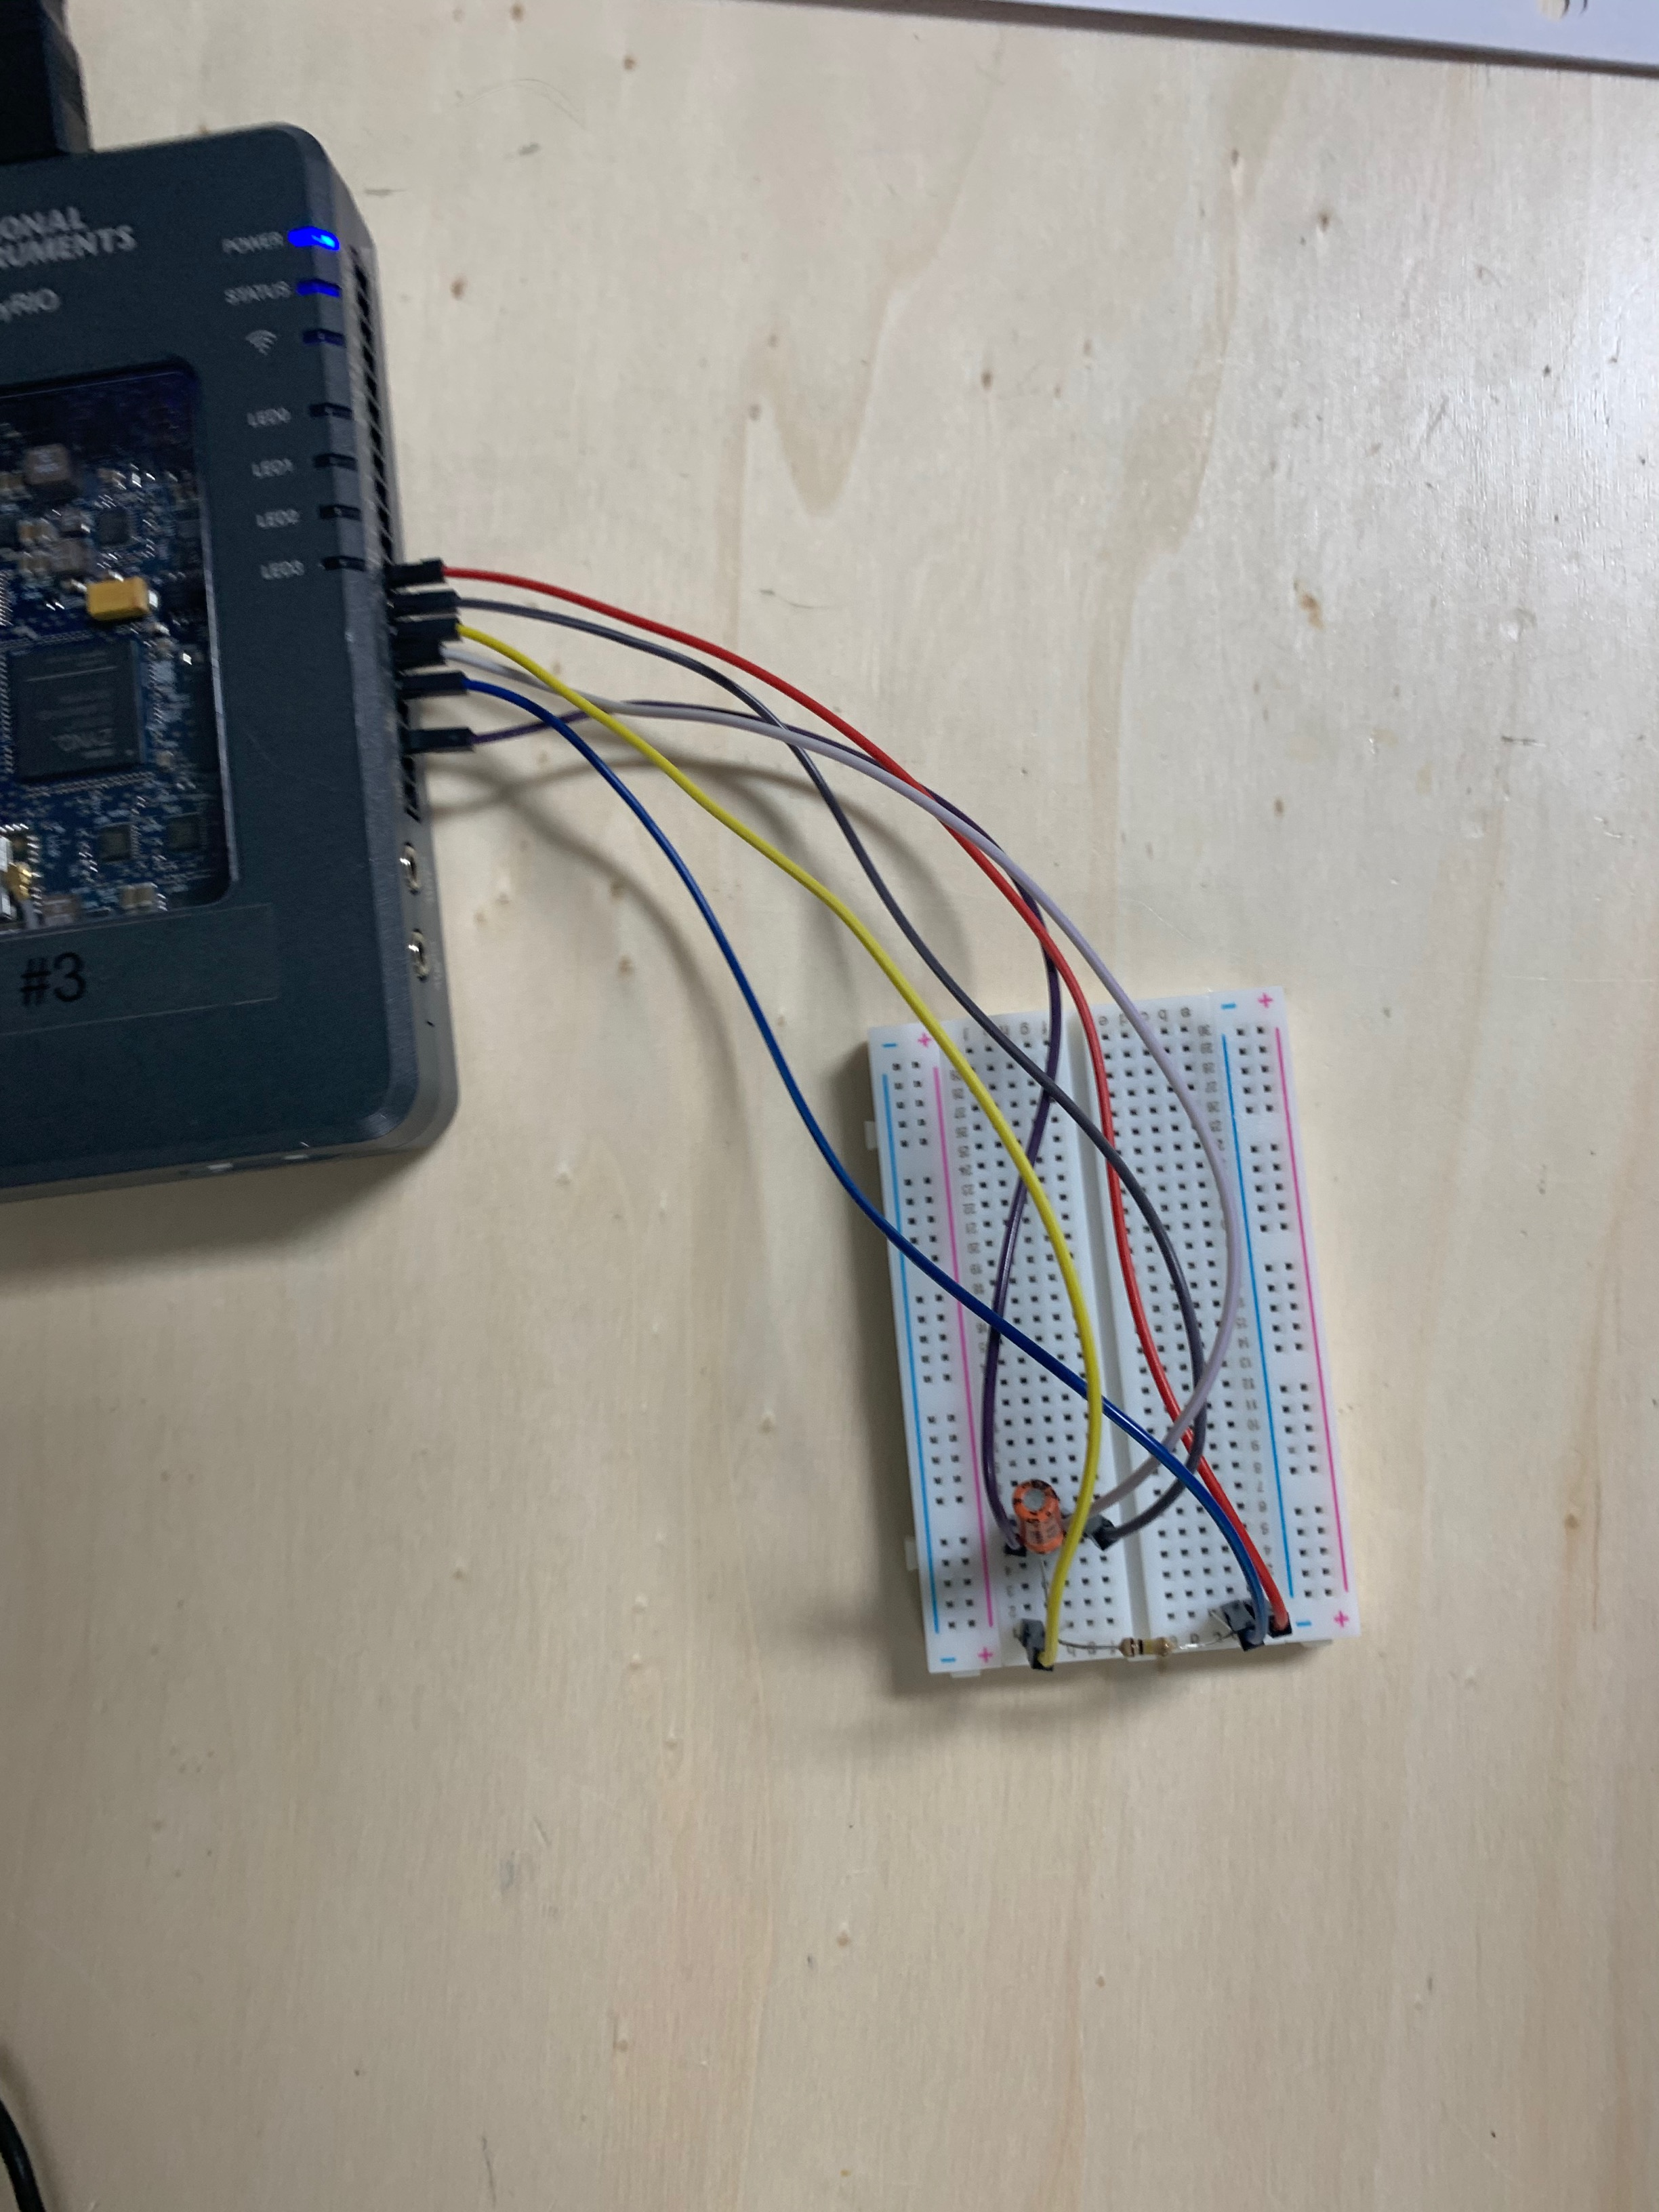
\includegraphics[width=.9\linewidth]{figures/RC.PNG}
	\caption{RC Circuit}
	\label{fig:circuit}
\end{figure}

\begin{figure}[bt]
	\centering
	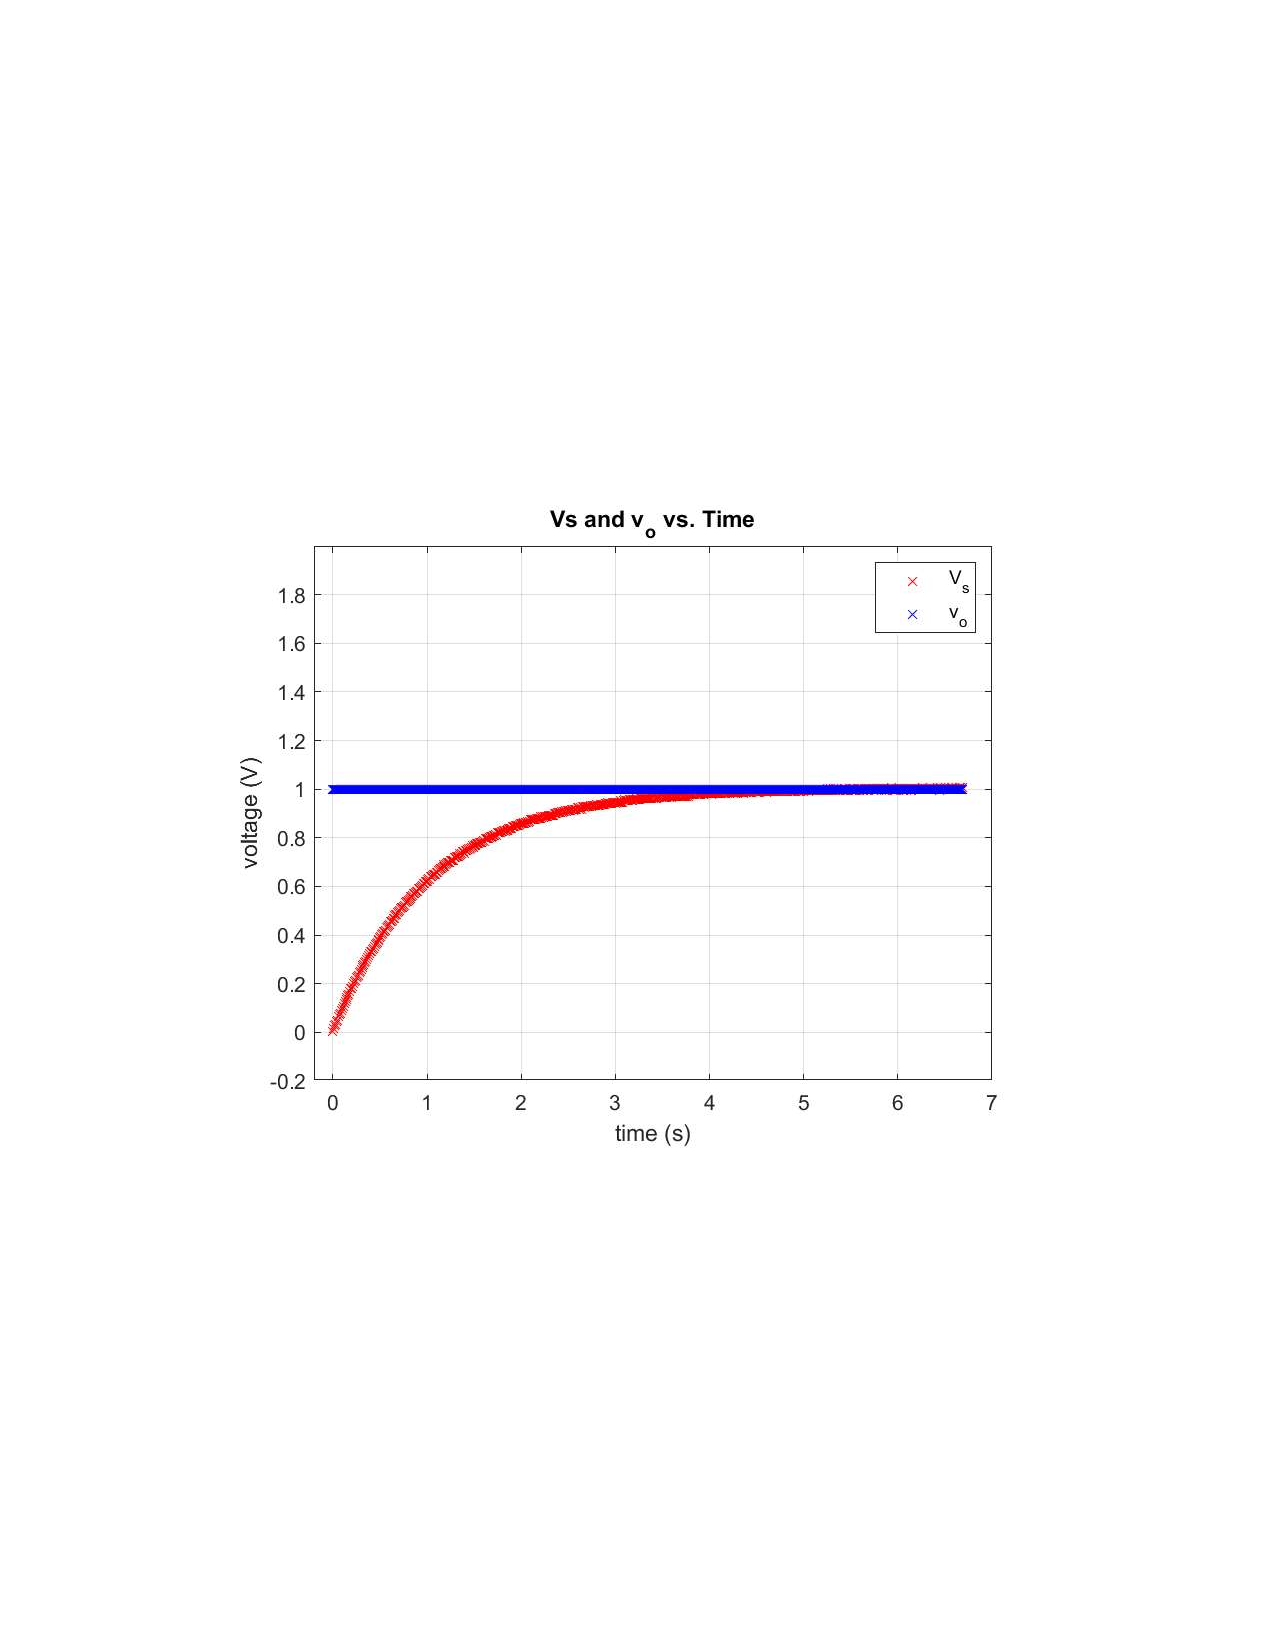
\includegraphics[width=.9\linewidth]{figures/RCgraph.pdf}
	\caption{Voltage vs. Time}
	\label{fig:RCgraph}
\end{figure}
\begin{figure}[bt]
	\centering
	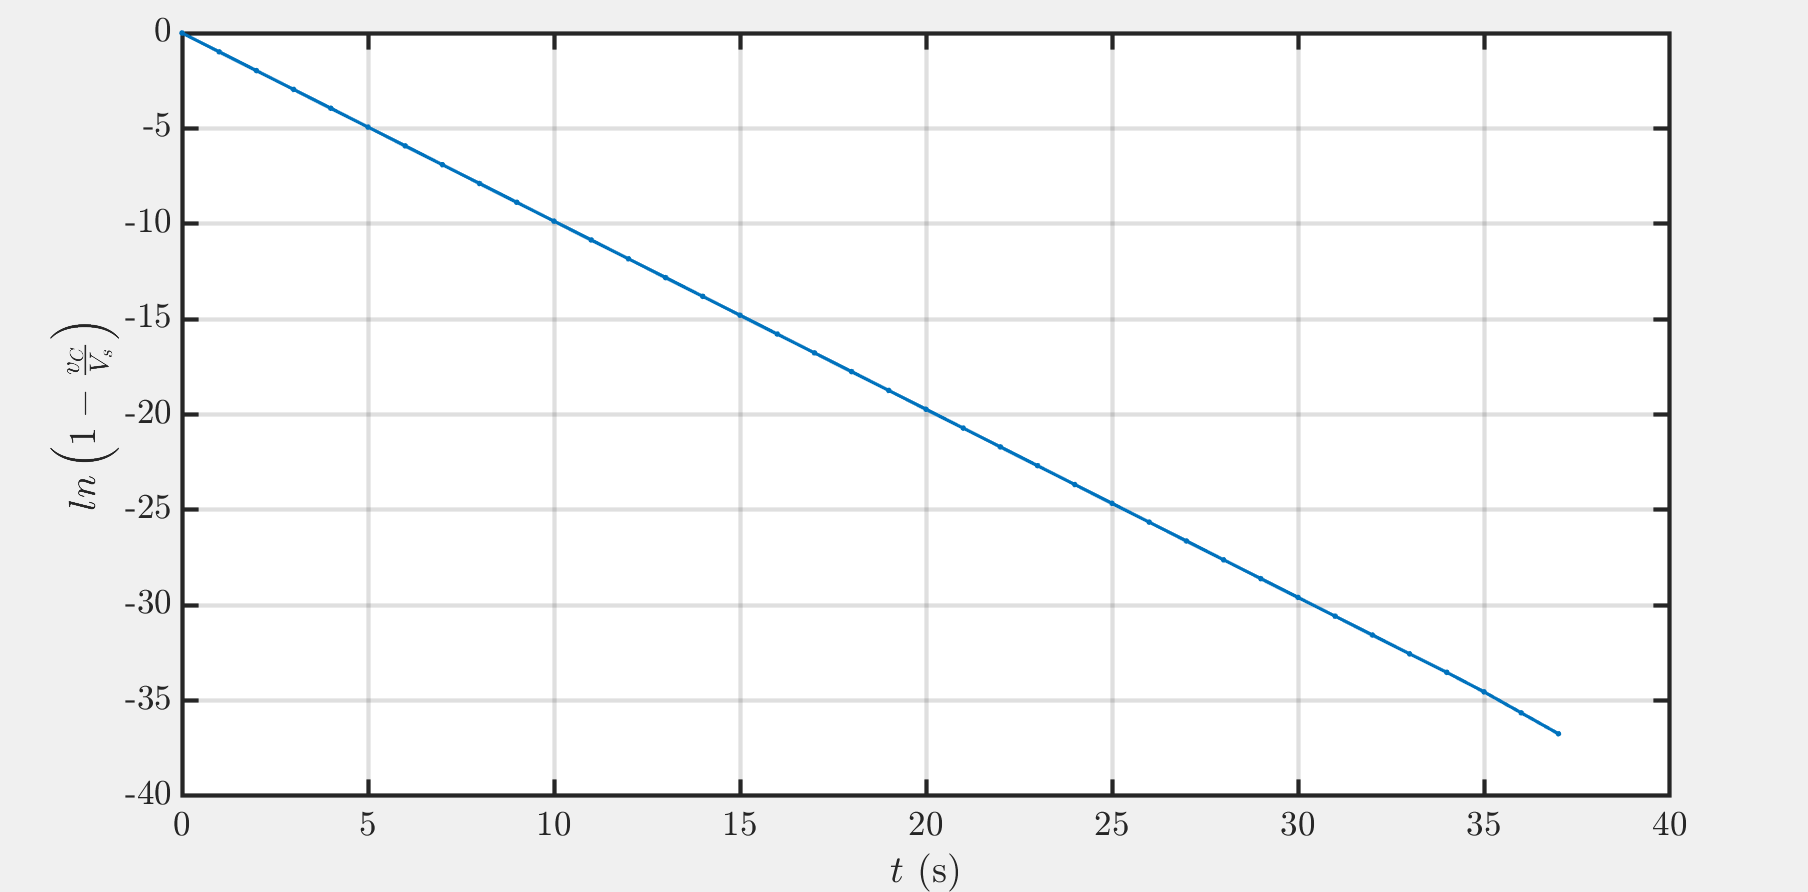
\includegraphics[width=.9\linewidth]{figures/Linear.PNG}
	\caption{Linearized data}
	\label{fig:Linear}
\end{figure}

\begin{figure}[bt]
	\centering
	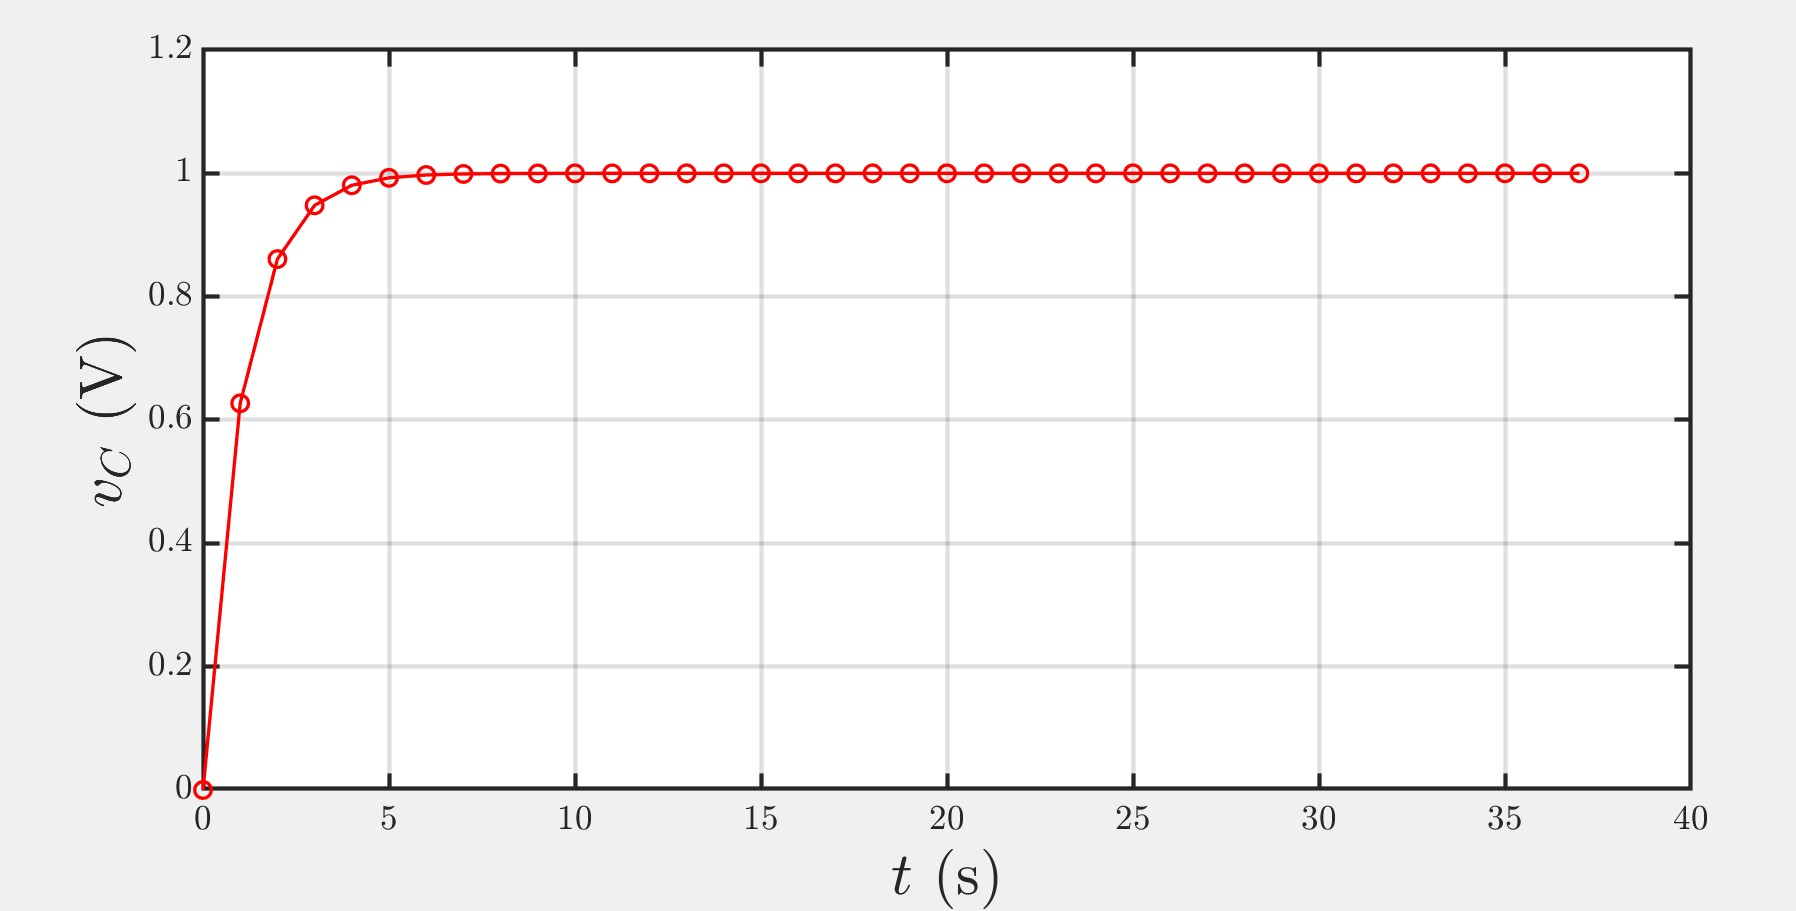
\includegraphics[width=.9\linewidth]{figures/vc.jpg}
	\caption{v_{c} vs. Time}
	\label{fig:VC}
\end{figure}

\begin{table}[bt]
	\begin{tabularx}{1\linewidth}{ lXX }
		\hline
		 & \textbf{R (kΩ) } & \textbf{C (µF)} \\
		\hline
		Nominal & $100$ & $10$ \\
		Measured & $99.4$ & $10.2$ \\
		\hline
	\end{tabularx}
	\caption{Multimeter Measurements}
	\label{tab:TAB1}
\end{table}
\section{Discussion}


``This is the section of the paper for you to show off your understanding of the data. You should summarize what you found. Explain how this relates to what others have found. Explain the implications.''

\section{Equations}

\begin{align*}
	V_{c}(t) = V_{s}
	\left(
	1- e^\frac{-t}{\tau}
	\right)
\end{align*}

\begin{align*}
	\tau = \frac{-t}{ln
	\left(
	1- \frac{V_{c}\left(
	t
	\right)}{V_{s}\left(
	t
	\right)}}
        \right)
\end{align*}

\section{Author Contributions}
Alex created the voltage versus time graph. He also wrote the abstract, the introduction, and wrote the materials and methods section. Austin applied the photos and the table. Irfan made the circuit diagram







\end{document}  
